\section{Convex Model Predictive Control (MPC)}

\begin{itemize}
    \item We have already learned LQR, which is very powerful. But we often need to reason about constraints, boxed, linear, etc, such as torque limits.
    \item Constraints break the Riccati solution, we can't directly use the feedback matrix, but we can still solve the QP online. Convex MPC has gotten popular as computers have gotten faster. Earlier in the 70s in chemical engineering where the Dynamics like solving it in 30 seconds was real time on a chemical plan, now we do it at kilohertz rates on robots.
\end{itemize}

\subsection{Background: Convexity}

\subsubsection{Convex Set}
A line connecting any two points in the set is also also contained in the set:
\begin{center}
    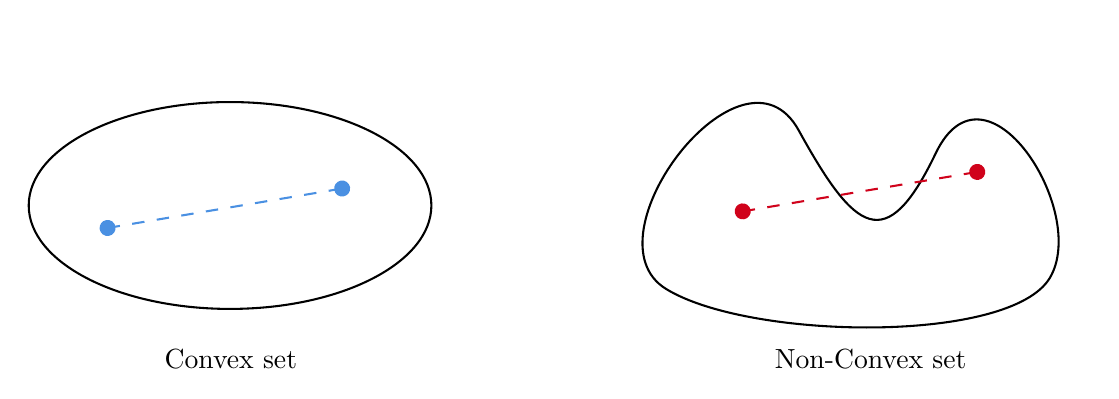
\begin{tikzpicture}[x=0.75pt,y=0.75pt,yscale=-1,xscale=1]
        \draw   (78,133.84) .. controls (78,106.31) and (121.43,84) .. (175,84) .. controls (228.57,84) and (272,106.31) .. (272,133.84) .. controls (272,161.36) and (228.57,183.67) .. (175,183.67) .. controls (121.43,183.67) and (78,161.36) .. (78,133.84) -- cycle ;
        \draw [color={rgb, 255:red, 74; green, 144; blue, 226 }  ,draw opacity=1 ] [dash pattern={on 4.5pt off 4.5pt}]  (116,144.67) -- (170.15,135.57) -- (229,125.67) ;
        \draw [shift={(229,125.67)}, rotate = 350.46] [color={rgb, 255:red, 74; green, 144; blue, 226 }  ,draw opacity=1 ][fill={rgb, 255:red, 74; green, 144; blue, 226 }  ,fill opacity=1 ][line width=0.75]      (0, 0) circle [x radius= 3.35, y radius= 3.35]   ;
        \draw [shift={(116,144.67)}, rotate = 350.46] [color={rgb, 255:red, 74; green, 144; blue, 226 }  ,draw opacity=1 ][fill={rgb, 255:red, 74; green, 144; blue, 226 }  ,fill opacity=1 ][line width=0.75]      (0, 0) circle [x radius= 3.35, y radius= 3.35]   ;
        \draw   (449,97.67) .. controls (476,146.67) and (491,158.67) .. (515,108.67) .. controls (539,58.67) and (589,136.67) .. (570,168.67) .. controls (551,200.67) and (425,198.67) .. (385,174) .. controls (345,149.33) and (422,48.67) .. (449,97.67) -- cycle ;
        \draw [color={rgb, 255:red, 208; green, 2; blue, 27 }  ,draw opacity=1 ] [dash pattern={on 4.5pt off 4.5pt}]  (422,136.67) -- (476.15,127.57) -- (535,117.67) ;
        \draw [shift={(535,117.67)}, rotate = 350.46] [color={rgb, 255:red, 208; green, 2; blue, 27 }  ,draw opacity=1 ][fill={rgb, 255:red, 208; green, 2; blue, 27 }  ,fill opacity=1 ][line width=0.75]      (0, 0) circle [x radius= 3.35, y radius= 3.35]   ;
        \draw [shift={(422,136.67)}, rotate = 350.46] [color={rgb, 255:red, 208; green, 2; blue, 27 }  ,draw opacity=1 ][fill={rgb, 255:red, 208; green, 2; blue, 27 }  ,fill opacity=1 ][line width=0.75]      (0, 0) circle [x radius= 3.35, y radius= 3.35]   ;
        \draw (142,202) node [anchor=north west][inner sep=0.75pt]   [align=left] {Convex set};
        \draw (436,202) node [anchor=north west][inner sep=0.75pt]   [align=left] {Non-Convex set};
    \end{tikzpicture}
\end{center}

Standard Example:
\begin{itemize}
    \item Linear subspace: $Ax=b$.
    \item Half space/box/polytope: $Ax = b$.
    \item Ellipsoids: $x^TPx\le 1,P\succ 0$.
    \item Cones: $\lVert x_{2:n} \rVert _2\le x_1$ (second-order cone, a.k.a. standard ice cream cone).
\end{itemize}

\subsubsection{Convex Function}
A function $f(x): \mathbb{R}^n\to \mathbb R$ who's epigraph is a convex set: (For twice differentiable functions, you can say its hessian is PD or something)
\begin{center}
    \tikzset{
        pattern size/.store in=\mcSize,
        pattern size = 5pt,
        pattern thickness/.store in=\mcThickness,
        pattern thickness = 0.3pt,
        pattern radius/.store in=\mcRadius,
        pattern radius = 1pt}
    \makeatletter
    \pgfutil@ifundefined{pgf@pattern@name@_820zad5vl}{
        \pgfdeclarepatternformonly[\mcThickness,\mcSize]{_820zad5vl}
        {\pgfqpoint{0pt}{0pt}}
        {\pgfpoint{\mcSize+\mcThickness}{\mcSize+\mcThickness}}
        {\pgfpoint{\mcSize}{\mcSize}}
        {
            \pgfsetcolor{\tikz@pattern@color}
            \pgfsetlinewidth{\mcThickness}
            \pgfpathmoveto{\pgfqpoint{0pt}{0pt}}
            \pgfpathlineto{\pgfpoint{\mcSize+\mcThickness}{\mcSize+\mcThickness}}
            \pgfusepath{stroke}
        }}
    \makeatother
    \tikzset{
        pattern size/.store in=\mcSize,
        pattern size = 5pt,
        pattern thickness/.store in=\mcThickness,
        pattern thickness = 0.3pt,
        pattern radius/.store in=\mcRadius,
        pattern radius = 1pt}
    \makeatletter
    \pgfutil@ifundefined{pgf@pattern@name@_uy5nsnazh}{
        \pgfdeclarepatternformonly[\mcThickness,\mcSize]{_uy5nsnazh}
        {\pgfqpoint{0pt}{0pt}}
        {\pgfpoint{\mcSize+\mcThickness}{\mcSize+\mcThickness}}
        {\pgfpoint{\mcSize}{\mcSize}}
        {
            \pgfsetcolor{\tikz@pattern@color}
            \pgfsetlinewidth{\mcThickness}
            \pgfpathmoveto{\pgfqpoint{0pt}{0pt}}
            \pgfpathlineto{\pgfpoint{\mcSize+\mcThickness}{\mcSize+\mcThickness}}
            \pgfusepath{stroke}
        }}
    \makeatother
    \begin{tikzpicture}[x=0.75pt,y=0.75pt,yscale=-1,xscale=1]
        \draw  (79,189.17) -- (248,189.17)(163.88,73.5) -- (163.88,230.17) (241,184.17) -- (248,189.17) -- (241,194.17) (158.88,80.5) -- (163.88,73.5) -- (168.88,80.5)  ;
        \draw [pattern=_820zad5vl,pattern size=6pt,pattern thickness=0.75pt,pattern radius=0pt, pattern color={rgb, 255:red, 0; green, 0; blue, 0}]   (222,107.33) .. controls (219,140.33) and (188,197.33) .. (164.5,196.33) .. controls (141,195.33) and (111,144.33) .. (105,111.33) ;
        \draw  (392,189.17) -- (561,189.17)(476.88,73.5) -- (476.88,230.17) (554,184.17) -- (561,189.17) -- (554,194.17) (471.88,80.5) -- (476.88,73.5) -- (481.88,80.5)  ;
        \draw [pattern=_uy5nsnazh,pattern size=6pt,pattern thickness=0.75pt,pattern radius=0pt, pattern color={rgb, 255:red, 0; green, 0; blue, 0}]   (563,107.83) .. controls (560,140.83) and (529,197.83) .. (505.5,196.83) .. controls (482,195.83) and (474,160.83) .. (466,138.83) .. controls (458,116.83) and (450,188.83) .. (430,143.83) .. controls (410,98.83) and (411,185.83) .. (390,106.83) ;
        \draw (110,239) node [anchor=north west][inner sep=0.75pt]   [align=left] {Convex function};
        \draw (409,239) node [anchor=north west][inner sep=0.75pt]   [align=left] {Non-Convex function};
    \end{tikzpicture}
\end{center}
Standard Example:
\begin{itemize}
    \item Linear: $f(x)=c^Tx$.
    \item Quadratic: $f(x) =\frac{1}{2}x^TQx +q^Tx ,Q\succ0$.
    \item (Any) Norms: $f(x)=\left| x \right|$.
\end{itemize}

\subsection{Convex Optimizaiton Problem}
Minimizing a convex function over a convex set. Standard Example:
\begin{table}[H]
    \centering
    \caption{These problems are in a hierarchy structure, a.k.a. a top-down containment relationship.}
    \begin{tabular}{ccc}
    \hline
    Convex Problem                      & Cost Function & Constraint Set \\ \hline
    Linear Program (LP)                 & Linear        & Linear         \\
    Quadratic Program (QP)              & Quadratic     & Linear         \\
    Quadratically-Constrained QP (QCQP) & Quadratic     & Ellipsoidal    \\
    Second-order Cone Program (SOCP)    & Linear        & Cone           \\ \hline
    \end{tabular}
\end{table}
Convex optimization problems have some advantages:
\begin{itemize}
    \item Convex problems don't have any spurious local optima that satisfy KKT conditions. If you find a local KKT solution, you have the global optimum.
    \item Practically, Newton's method converges really fast, and reliably (5 to 10 iterations at most). Therefore, it can bound solution time for real-time control.
\end{itemize}

\subsection{Convex MPC}
Think about this as ``constrained LQR''. Remember from DP, if we have a cost-to-go function, we can get $u$ by solving a one-step problem:
\begin{equation}
    \begin{array}{rl}
        u_{k}(x) &= \arg\min_{u\in\mathcal{U}}\left[l\left(x,u\right)+V_{k+1}\left(f\left(x,u\right)\right)\right] \\[6.18pt]
        &=\min_u\frac{1}{2}u^TRu+\left( A_{k}x_{k}+B_{k}u \right) ^TP_{k+1}\left( A_{k}x_{k}+B_{k}u \right)
    \end{array}
\end{equation}

We can add constraints on $u$ to this one-step problem, but this will perform poorly because $V(x)$ was computed without constraints, if we add constraints to backward pass, there is no analytical solution. The detailed explanation is as follows:

\begin{itemize}
    \item 在Lecture 8的通过动态规划推导LQR的过程中，得知系统的LQR最优反馈控制率$u$是由最小化系统的Cost-to-Go函数$V(x)$得到的，这个过程我们实际上是对$V(x)$对$u$求梯度令其等于0，得到系统的$u$，因此我们解的是一个不考虑$u$约束的最小化$V$的问题来得到$u$，假如要解一个带$u$约束的最小化问题，则，此问题无法写出解析解（因为在推导的过程也不知道实际的$u$会是一个什么约束），也就无法进行下一步的迭代。因此，想要在DP或者Riccati迭代中处理$u$的约束，是比较困难的（当然可以通过罚函数法或者增广拉格朗日法把约束变成Cost，后文DDP中会讲）。
    \item 在DP或者Riccati中，处理$x$的约束就更难了，$x$在整个推导过程中，不像$u$那样是直接解最优化方程得到的，而是解出$u$之后再通过$x_1$前向rollout得到的，因此这个过程很不直接，想要约束$x$难度更大.
    \item 但是，假如通过QP来解LQR问题，关于LQR问题中的所有$x,u$的线性约束都可以转成标准的$Cx\le d$的标准形式，这样仍然是一个标准的QP问题（虽然要在QP中处理约束了，但是还是有成熟的求解器，我们自己也可以基于增广拉格朗日实现简单的），在求解流程上并无区别。
    \item 因此，目前主流的Convex MPC都是通过转化成QP的形式，再利用QP形式KKT系统Hessian矩阵的稀疏性，加速QP过程的求解，也可以做到几千hz
    \item As for adding constraints to the one-step problem (such as riccati recursion and dynamic programming). The $u_{\arg\min}$ plugged into next $K$ matrix will clip (affect) the $K$ matrix (recall Equ. \eqref{equ:lqr-dp}), further affect the cost-to-go function $V$. However, it is obvious that $V(x)$ is independent of control input $u$, it is only dependent of state $x$. Therefore, the $V$ should be the same whether the constraint is applied or not. But the applied constraint certainly will affect $V$.
    \item  As for the LQR-QP, if we add the constraints to the QP problem, the constraints act as global constraints, making each step have good consistency.
    \item However, adding constraints to QP problem leads to bad computational complexity, on the other hand, adding constraints to one-step problem is sketchy. There is a trade off between steps and the accuracy of the solution. There's no reason I can't add more steps to the one-step problem. The number of steps is called ``horizon'', denoted as $H$, we add constraints to the QP inside the horizon.
\end{itemize}

% 进一步影响到V函数，而显然V函数与输入无关，至于状态有关，因此无论是否加约束，求出来的V应该是一样的，而加了约束后是不一样的.如果是在LQR的QP问题中加入约束,相当于是全局的约束,如果在每一步中加入约束,那么每一步的求解都是矛盾的,但是在LQR的QP中加入约束,整个问题就很庞大,如果只在一步中加入QP,又很粗糙,于是取一个折中方案,就是给一个在1~N之间的数H作为horizon,在这个horizon中对QP问题添加约束.

\begin{equation}
    \begin{aligned}
        \min_{\substack{x_{1:N}\\u_{1:N-1}}}J=\sum_{k=1}^{N-1}{\frac{1}{2}x_{k}^{T}Q_kx_k+\frac{1}{2}u_{k}^{T}R_ku_k}+\underset{\text{LQR cost-to-go}}{\underbracket{\frac{1}{2}x_{H}^{T}P_Hx_H}} \\
        \text{s.t.} \qquad x_{k+1} = A_k x_k + B_k u_k \\
        x_k\in \mathcal{X} \\
        u_k\in \mathcal{U} \\
        \mathcal{X} \text{ and } \mathcal{U} \text{ are convex.}
    \end{aligned}
\end{equation}

There are some notes:
\begin{itemize}
    \item With no additional constraints, MPC (receding horizon) exactly matches LQR for any $H$.
    \item Intuition: explicit constrained optimization over first $H$ steps gets the state close enough to the reference that the constraints are no longer active and LQR solution/cost-to-go is valid further into the future.
    \item The selection of $H$ is very important. For example, control input is easily saturated when the system is heavily disturbed, under this circumstance, MPC works, limiting the control input $u$ in a feasible range. Till the horizon is about to the end, you don't need too much control input to control the system, this is when LQR works. So MPC needs LQR's cost-to-go to estimate the future cost. Basically, the longer horizon the better performance, but needs trade off. 
    \item If I have a constraint value function(cost-to-go), then MPC's horizon can be set to 1.
    \item The better I make the value function the shorter the horizon could be. The worse the value function is, the bigger horizon to compensate. And this lets you get away with bad value function approximations. There's many extensions of these kind of ideas by learning a value function approximation with a neural net or whatever and stick that in to an MPC controller in place of this LQR one.
    \item Convex MPC requires that the model must be linear, or even linear time-varying (such as along a reference trajectory). When it comes to nonlinear MPC, there will be many demons, but autonomous driving is always using a nonlinear model.
    \item Similar to dynamic programming, value function approximation at the tail is key to this MPC story, in fact like all the convergence proofs and theory of MPC have in them some kind of cost-to-go approximation at the tail and that's kind of a necessary thing to prove stability. So this is the right way to think about it.
\end{itemize}

In general, 
\begin{itemize}
    \item A good approximation of $V(x)$ is important for good performance.
    \item Better $V(x)$  shorter horizon.
    \item Longer $H$ leads to less reliance on $V(x)$.
\end{itemize}

\subsection{Example: Planar Quadrotor}

\begin{center}
    \tikzset{every picture/.style={line width=0.75pt}} %set default line width to 0.75pt        
    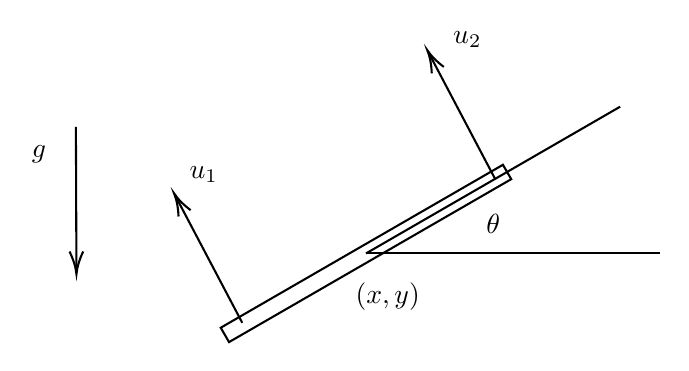
\begin{tikzpicture}[x=0.75pt,y=0.75pt,yscale=-1,xscale=1]
        \draw   (374.48,138.89) -- (238.52,217.39) -- (234.52,210.46) -- (370.48,131.96) -- cycle ;
        \draw    (445.92,174.67) -- (304.5,174.67) ;
        \draw    (426.97,103.96) -- (304.5,174.67) ;
        \draw    (244.88,208.09) -- (212.93,147.44) ;
        \draw [shift={(212,145.67)}, rotate = 62.22] [color={rgb, 255:red, 0; green, 0; blue, 0 }  ][line width=0.75]    (10.93,-3.29) .. controls (6.95,-1.4) and (3.31,-0.3) .. (0,0) .. controls (3.31,0.3) and (6.95,1.4) .. (10.93,3.29)   ;
        \draw    (366.88,139.09) -- (334.93,78.44) ;
        \draw [shift={(334,76.67)}, rotate = 62.22] [color={rgb, 255:red, 0; green, 0; blue, 0 }  ][line width=0.75]    (10.93,-3.29) .. controls (6.95,-1.4) and (3.31,-0.3) .. (0,0) .. controls (3.31,0.3) and (6.95,1.4) .. (10.93,3.29)   ;
        \draw    (164.73,113.65) -- (164.99,182.67) ;
        \draw [shift={(165,184.67)}, rotate = 269.78] [color={rgb, 255:red, 0; green, 0; blue, 0 }  ][line width=0.75]    (10.93,-3.29) .. controls (6.95,-1.4) and (3.31,-0.3) .. (0,0) .. controls (3.31,0.3) and (6.95,1.4) .. (10.93,3.29)   ;
        \draw (218,131.4) node [anchor=north west][inner sep=0.75pt]    {$u_{1}$};
        \draw (345,66.4) node [anchor=north west][inner sep=0.75pt]    {$u_{2}$};
        \draw (361,154.4) node [anchor=north west][inner sep=0.75pt]    {$\theta $};
        \draw (142,121.4) node [anchor=north west][inner sep=0.75pt]    {$g$};
        \draw (298,187.4) node [anchor=north west][inner sep=0.75pt]    {$( x, y)$};
    \end{tikzpicture}
\end{center}

The dynamics of the planar quadrotor is
\begin{equation}
    \begin{array}{rl}
        m\ddot{x}&=-(u_1+u_2)\sin(\theta)\\[6.18pt]
        m\ddot{y}&=(u_1+u_2)\cos(\theta)-mg\\[6.18pt]
        J\ddot{\theta}&=\frac{1}{2}l(u_2-u_1)
    \end{array}
\end{equation}

Linearize about hover, when $u_1=u_2=\frac{1}{2}mg$:
% \begin{equation}
%     \begin{array}{rl}
%         \Delta \ddot x &\approx -g\Delta \theta \\[6.18pt]
%         \Delta \ddot y &\approx \frac{1}{m}(\Delta u_1+\Delta u_2) \\[6.18pt]
%         \Delta \ddot \theta &\approx \frac{1}{J}\frac{l}{2}(\Delta u_1-\Delta u_2)
%     \end{array}
% \end{equation}
\begin{align*}
    u_1 = u_2 = \frac{1}{2} mg,  \ \theta = 0\text{ (\text{Hover})} \\          
    \Rightarrow
    \begin{cases}
        \Delta \ddot x      & \approx \frac{\partial f_1(x,y,\theta,u)}{\partial u_1}|_{\text{Hover}} \Delta u_1 + \frac{\partial f_1(x,y,\theta,u)}{\partial u_2}|_{\text{Hover}}\Delta u_2 + \frac{\partial f_1(x,y,\theta,u)}{\partial \theta}|_{\text{Hover}}\Delta \theta  \\
                            & \approx\frac{1}{m}\left(-sin(\theta)|_{\text{Hover}}\Delta u_1-sin(\theta)|_{\text{Hover}}\Delta u_2 -(u_1+u_2)cos(\theta)|_{\text{Hover}}\Delta \theta\right)\approx-g \Delta \theta                                                                                      \\
        \Delta \ddot y      & \approx \frac{\partial f_2(x,y,\theta,u)}{\partial u_1}|_{\text{Hover}} \Delta u_1 + \frac{\partial f_2(x,y,\theta,u)}{\partial u_2}|_{\text{Hover}}\Delta u_2 + \frac{\partial f_2(x,y,\theta,u)}{\partial \theta}|_{\text{Hover}}\Delta \theta  \\
                            & \approx \frac{1}{m}\left(cos(\theta)|_{\text{Hover}}\Delta u_1+cos(\theta)|_{\text{Hover}}\Delta u_2 -(u_1+u_2)sin(\theta)|_{\text{Hover}}\Delta \theta\right)\approx \frac{1}{m} (\Delta u_1 + \Delta u_2)                                                                \\
        \Delta \ddot \theta & \approx \frac{1}{J} \frac{l}{2}(\Delta u_2 - \Delta u_1)
    \end{cases}                                       \\
\end{align*}

The state space equation is
\begin{equation}
    \underset{\dot{x}}{\underbrace{\left[ \begin{array}{c}
        \Delta \dot{x}\\
        \Delta \dot{y}\\
        \Delta \dot{\theta}\\
        \Delta \ddot{x}\\
        \Delta \ddot{y}\\
        \Delta \ddot{\theta}\\
    \end{array} \right] }}=\underset{A}{\underbrace{\left[ \begin{matrix}
        0&		0&		0&		1&		0&		0\\
        0&		0&		0&		0&		1&		0\\
        0&		0&		0&		0&		0&		1\\
        0&		0&		-g&		0&		0&		0\\
        0&		0&		0&		0&		0&		0\\
        0&		0&		0&		0&		0&		0\\
    \end{matrix} \right] }}\underset{x}{\underbrace{\left[ \begin{array}{c}
        \Delta x\\
        \Delta y\\
        \Delta \theta\\
        \Delta \dot{x}\\
        \Delta \dot{y}\\
        \Delta \dot{\theta}\\
    \end{array} \right] }}+\underset{B}{\underbrace{\left[ \begin{matrix}
        0&		0\\
        0&		0\\
        0&		0\\
        0&		0\\
        \frac{1}{m}&		\frac{1}{m}\\
        -\frac{l}{2J}&		\frac{l}{2J}\\
    \end{matrix} \right] }}\underset{u}{\underbrace{\left[ \begin{array}{c}
        \Delta u_1\\
        \Delta u_2\\
    \end{array} \right] }}
\end{equation}

The cost function:
% \begin{equation}
%     J=\sum_{k=1}^{H-1}{\left[ \frac{1}{2}\left( x_k-x_{\text{ref}} \right) ^TQ\left( x_k-x_{\text{ref}} \right) +\frac{1}{2}\Delta u_{n}^{T}R\Delta u_n \right]}+\frac{1}{2}\left( x_H-x_{\text{ref}} \right) ^TQ\left( x_H-x_{\text{ref}} \right) 
% \end{equation}
\begin{align*}
    \min_{x_{1:H}, u_{1:H-1}}   & \sum_{k=1}^{H-1} [\frac{1}{2} (x_k-x_{ref})^T Q_k (x_k-x_{ref}) + \frac{1}{2} u_k^T R_k u_k] + (x_H-x_{ref})^T P (x_H-x_{ref}) \\
    = \min_{x_{1:H}, u_{1:H-1}} & \sum_{k=1}^{H-1} [\frac{1}{2} x_k^T Q_k x_k + \frac{1}{2} u_k^T R_k u_k - (Q_kx_{ref})^Tx_k] + x_H^T P x_H - (Px_{ref})^Tx_H \\
                                & x_{min}\leq x \leq x_{max} \ \  u_{min}\leq u \leq u_{max}
\end{align*}

This can be converted to a standard QP, we stack the decision variables as we did before. We use OSQP solver, $N=20, \text{dim}(x)=6, \text{dim}(u)=2$, actually, the decision variables are $x_{2:21}, u_{1:20}$, so the dimension of $z$ is 160. OSQP only supports inequality constraints $\text{lower bound} \le Dz \le \text{upper bound}$, therefore all the equality constraints have to be converted to inequality constraints, in which lower bound = upper bound.

\begin{gather*}
    z=\begin{bmatrix}
    u_{1}\\
    x_{2}\\
    u_{2}\\
    \vdots \\
    u_{20}\\
    x_{21}
    \end{bmatrix}\\
    H=\begin{bmatrix}
    R & 0 & \cdots  & 0 & \cdotp  & 0 & 0\\
    0 & Q & \cdots  & 0 & \cdotp  & 0 & 0\\
     &  & \cdotp  &  &  &  & \\
    0 & 0 & \cdots  & Q & \cdotp  & 0 & 0\\
    \cdotp  & \cdotp  & \cdots  & \cdotp  & \cdotp  & \cdotp  & 0\\
    0 & 0 & \cdots  & 0 & \cdotp  & R & 0\\
    0 & 0 & \cdots  & 0 & \cdotp  & 0 & P
    \end{bmatrix} \in \mathbb{R}^{160\times 160}
\end{gather*}

\begin{align}     D &= \begin{bmatrix}         B_1 & (-I)  & ...   & ...   & ...   & 0 \\         0   & A     & B     & (-I)& ...  & ...   & 0 \\         \   & \     & .     & \ \\         0   & 0     & ...   & ...& A_{20} & B_{20} & (-I)\\         -   & -     & -   & - & - & - &-\\           \   & \     &      & \ \\            &      &    &S_u  &  & \\                     \   & \     &      & \ \\  -   & -     & -   & - & - & -&-\\            \   & \     &      & \ \\             &      &    &S_{\theta}  &  & \\                       \   & \     &      & \ \\     \end{bmatrix} \in \mathbb R^{(120+40+20) \times 160}\\      lower &= \begin{bmatrix}         -A_1 x_1 \\         0 \\         . \\          0 \\         - \\         u_{min}\\         -\\         \theta_{min}     \end{bmatrix}\in\mathbb R^{(120+40+20)}     \ \          upper = \begin{bmatrix}         -A_1 x_1 \\         0 \\         . \\          0 \\         - \\         u_{min}\\         -\\         \theta_{min}     \end{bmatrix}\in\mathbb R^{(120+40+20)} \end{align}

其中，约束共有120个状态的等式约束（每条$x_{k+1}=A_kx_k+Bu_k$可以提供$dim(x)$个约束），40个关于输入$u$的约束（$u$一共有40个，其中$S_u \in \mathbb R^{40 \times 160}$是选择矩阵，使得$S_uz=u$），20个关于状态$\theta$的约束（其中$S_\theta \in \mathbb R^{20 \times 160}$是选择矩阵，使得$S_\theta z=\theta$）

在本问题中，轨迹上x(t) 所有点的参考值都是最终的那个目标点，而在作业HW2中，从起点到终点线性插值了一个函数，以插值后的函数用时间索引作为x(t)的参考。并且，问题的规模是一直不变的，一直会从当前时间对应的t往后走N步，就算到了终点也会继续往后，直到收敛。

reference point: $[0, 1]$

\begin{figure}[H]
    \centering
    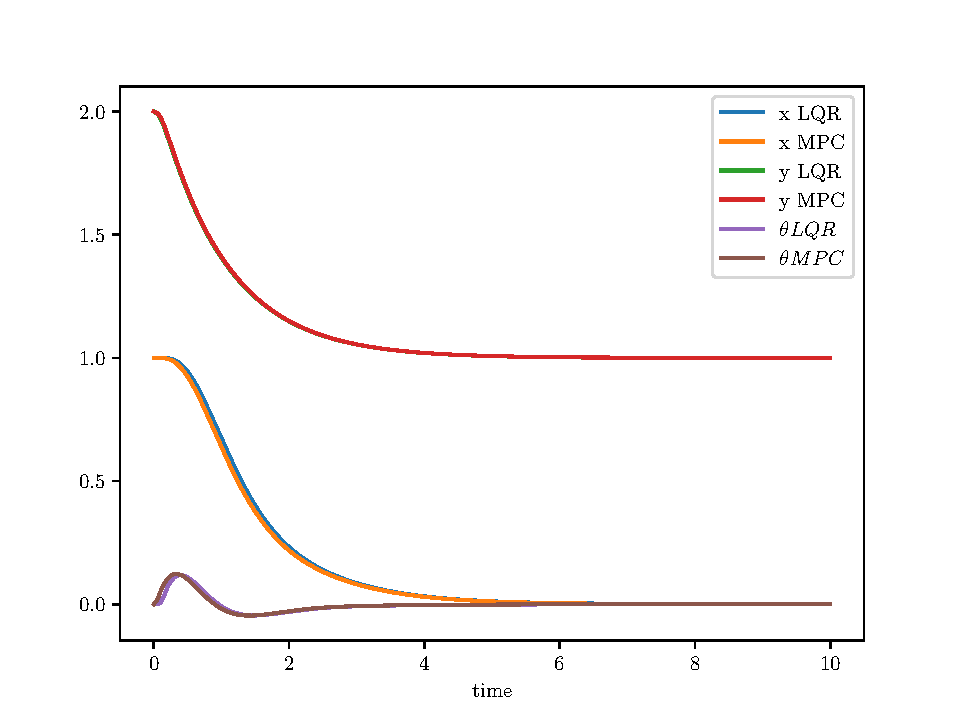
\includegraphics[scale=.75]{./tex/ch9/near_state.pdf}
    \caption{State variables starting at $[1, 2]$, with thrust limit constraints.}
\end{figure}

\begin{figure}[H]
    \centering
    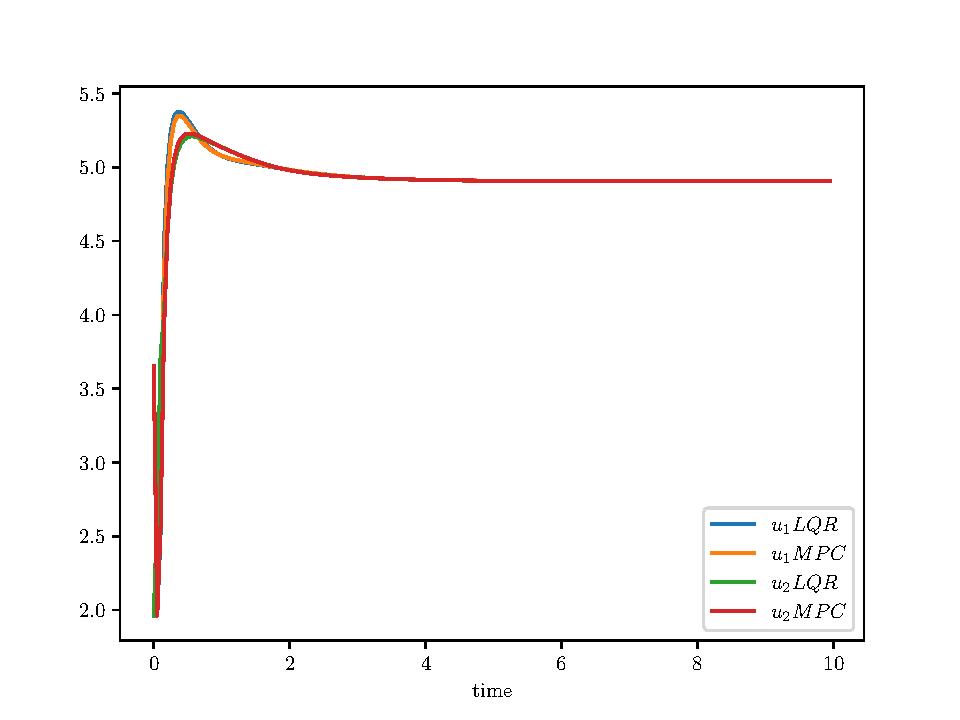
\includegraphics[scale=.75]{./tex/ch9/near_control.pdf}
    \caption{Control inputs starting at $[1, 2]$, with thrust limit constraints.}
\end{figure}

So far, it is good for both method.

\begin{figure}[H]
    \centering
    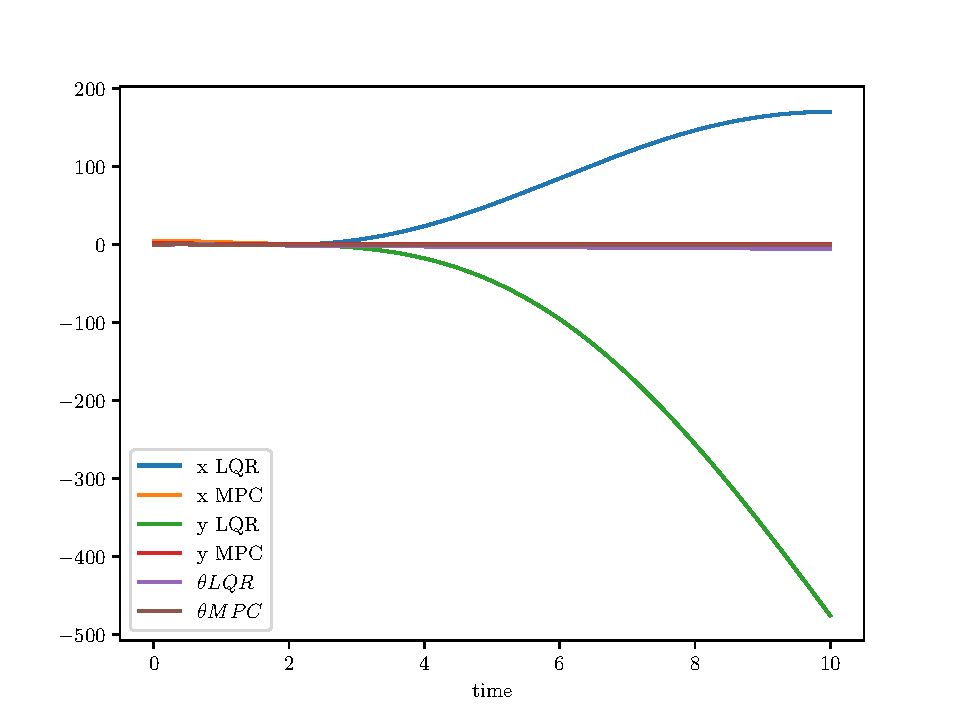
\includegraphics[scale=.75]{./tex/ch9/far_state.pdf}
    \caption{State variables starting at $[5, 2]$, with thrust limit constraints.}
\end{figure}
\begin{figure}[H]
    \centering
    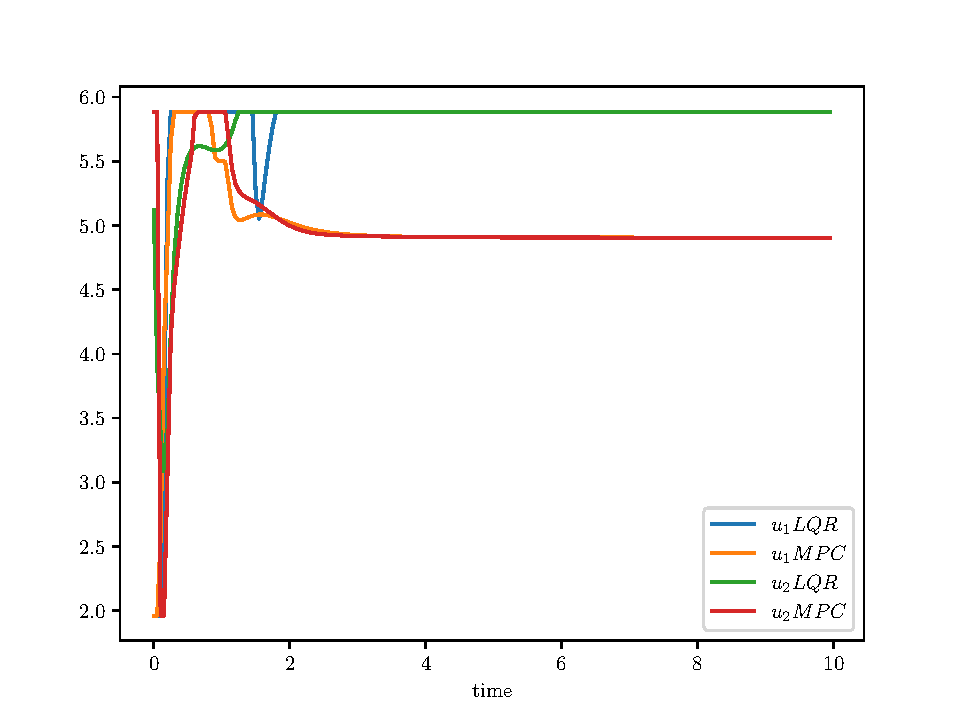
\includegraphics[scale=.75]{./tex/ch9/far_control.pdf}
    \caption{Control inputs starting at $[5, 2]$, with thrust limit constraints.}
\end{figure}

LQR blows up, while MPC works well. Why? Let's look at the $\theta$ and control input of LQR, since the linearization happens at a small neighbor of equilibrium point, the $\theta$ increased and get out of the small neighbor. Let's fix it.

\begin{figure}[H]
    \centering
    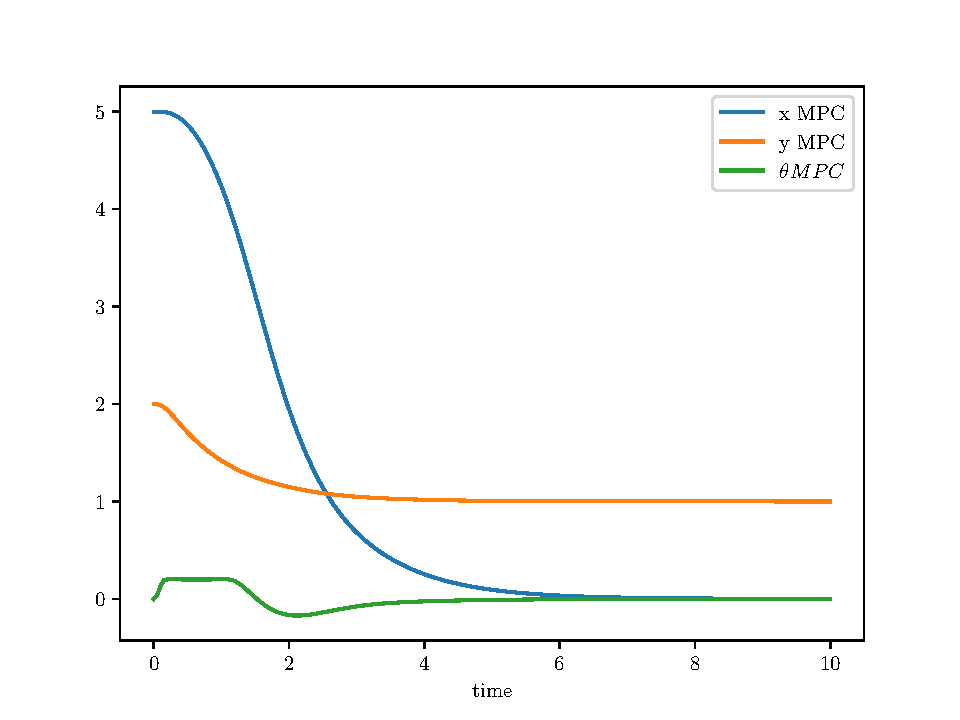
\includegraphics[scale=.75]{./tex/ch9/far_state_mpc.pdf}
    \caption{State variables starting at $[5, 2]$, with thrust limit and $\theta$ bound to $[-0.2, 0.2]$ constraints.}
\end{figure}
\begin{figure}[H]
    \centering
    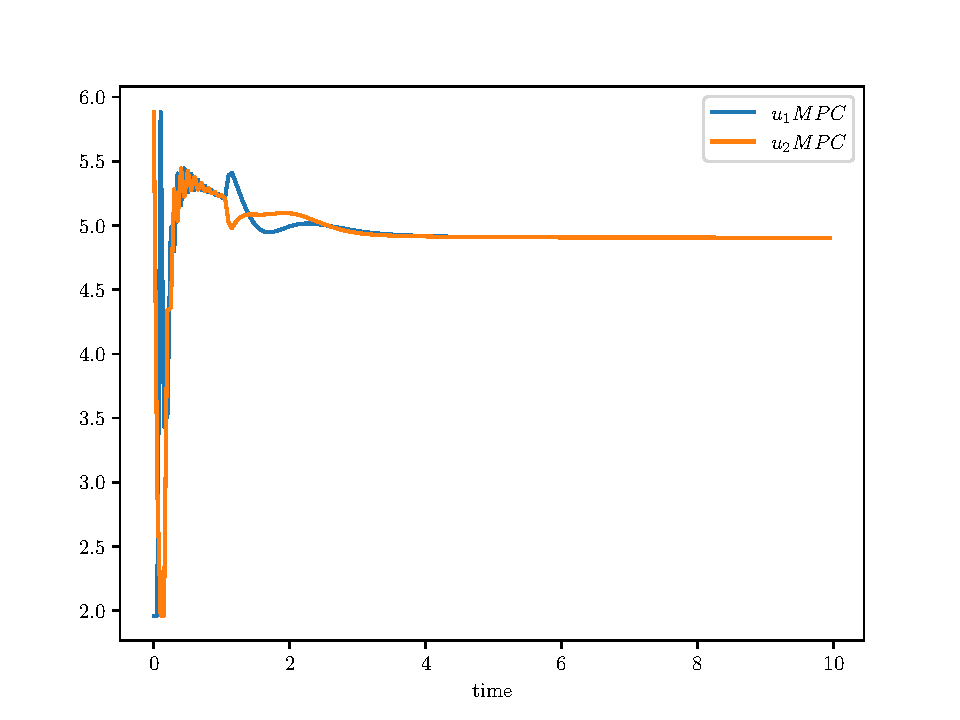
\includegraphics[scale=.75]{./tex/ch9/far_control_mpc.pdf}
    \caption{Control inputs starting at $[5, 2]$, with thrust limit and $\theta$ bound to $[-0.2, 0.2]$ constraints.}
\end{figure}

\subsection{Convex MPC Examples}
\begin{itemize}
    \item Rocket Landing
    Thrust vector constraints are conic:
    \begin{center}
        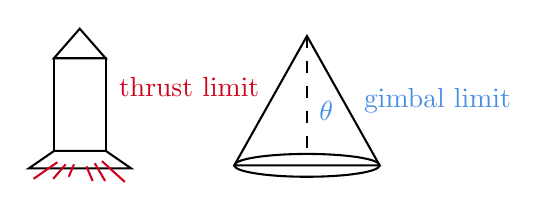
\begin{tikzpicture}[x=0.75pt,y=0.75pt,yscale=-1,xscale=1]
            \draw   (119.04,55) -- (131.57,69.33) -- (106.5,69.33) -- cycle ;
            \draw   (106.5,69.33) -- (131.57,69.33) -- (131.57,113.83) -- (106.5,113.83) -- cycle ;
            \draw   (94.44,122.33) -- (106.75,113.83) -- (131.53,113.83) -- (143.84,122.33) -- cycle ;
            \draw [color={rgb, 255:red, 208; green, 2; blue, 27 }  ,draw opacity=1 ][fill={rgb, 255:red, 208; green, 2; blue, 27 }  ,fill opacity=1 ]   (129.75,118.83) -- (140.75,128.83) ;
            \draw [color={rgb, 255:red, 208; green, 2; blue, 27 }  ,draw opacity=1 ][fill={rgb, 255:red, 208; green, 2; blue, 27 }  ,fill opacity=1 ]   (126.25,119.83) -- (131.25,128.33) ;
            \draw [color={rgb, 255:red, 208; green, 2; blue, 27 }  ,draw opacity=1 ][fill={rgb, 255:red, 208; green, 2; blue, 27 }  ,fill opacity=1 ]   (122.25,121.33) -- (125.25,128.33) ;
            \draw [color={rgb, 255:red, 208; green, 2; blue, 27 }  ,draw opacity=1 ][fill={rgb, 255:red, 208; green, 2; blue, 27 }  ,fill opacity=1 ]   (108.25,119.33) -- (96.75,127.33) ;
            \draw [color={rgb, 255:red, 208; green, 2; blue, 27 }  ,draw opacity=1 ][fill={rgb, 255:red, 208; green, 2; blue, 27 }  ,fill opacity=1 ]   (112.25,120.33) -- (106.25,127.33) ;
            \draw [color={rgb, 255:red, 208; green, 2; blue, 27 }  ,draw opacity=1 ][fill={rgb, 255:red, 208; green, 2; blue, 27 }  ,fill opacity=1 ]   (116.25,120.33) -- (113.75,126.33) ;
            \draw   (228.5,58.5) -- (263.5,120.83) -- (193.5,120.83) -- cycle ;
            \draw   (193.5,120.83) .. controls (193.5,117.79) and (209.17,115.33) .. (228.5,115.33) .. controls (247.83,115.33) and (263.5,117.79) .. (263.5,120.83) .. controls (263.5,123.87) and (247.83,126.33) .. (228.5,126.33) .. controls (209.17,126.33) and (193.5,123.87) .. (193.5,120.83) -- cycle ;
            \draw  [dash pattern={on 4.5pt off 4.5pt}]  (228.5,58.5) -- (228.5,115.33) ;
            \draw (233,88.4) node [anchor=north west][inner sep=0.75pt]  [color={rgb, 255:red, 74; green, 144; blue, 226 }  ,opacity=1 ]  {$\theta $};
            \draw (254.5,82) node [anchor=north west][inner sep=0.75pt]  [color={rgb, 255:red, 74; green, 144; blue, 226 }  ,opacity=1 ] [align=left] {gimbal limit};
            \draw (136.5,77) node [anchor=north west][inner sep=0.75pt]  [color={rgb, 255:red, 208; green, 2; blue, 27 }  ,opacity=1 ] [align=left] {thrust limit};
        \end{tikzpicture}
    \end{center}
    SpaceX and JPL Mars landing use SOCP-based MPC with linearized dynamics.
    \item Legged Robots
    Contact forces must obey ``friction come'' constraint:
    \begin{align}               \Vert b \Vert_2 \leq \mu n           \end{align}   
    
    \begin{center}
        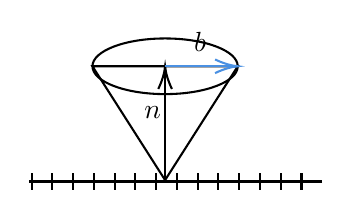
\begin{tikzpicture}[x=0.75pt,y=0.75pt,yscale=-1,xscale=1]
            \draw   (85,157.83) -- (120,103) -- (50,103) -- cycle ;
            \draw   (50,103) .. controls (50,95.59) and (65.67,89.59) .. (85,89.59) .. controls (104.33,89.59) and (120,95.59) .. (120,103) .. controls (120,110.41) and (104.33,116.41) .. (85,116.41) .. controls (65.67,116.41) and (50,110.41) .. (50,103) -- cycle ;
            \draw    (160.71,158.5) -- (19.29,158.5) (150.71,162.5) -- (150.71,154.5)(140.71,162.5) -- (140.71,154.5)(130.71,162.5) -- (130.71,154.5)(120.71,162.5) -- (120.71,154.5)(110.71,162.5) -- (110.71,154.5)(100.71,162.5) -- (100.71,154.5)(90.71,162.5) -- (90.71,154.5)(80.71,162.5) -- (80.71,154.5)(70.71,162.5) -- (70.71,154.5)(60.71,162.5) -- (60.71,154.5)(50.71,162.5) -- (50.71,154.5)(40.71,162.5) -- (40.71,154.5)(30.71,162.5) -- (30.71,154.5)(20.71,162.5) -- (20.71,154.5) ;
            \draw    (85,157.83) -- (85,105) ;
            \draw [shift={(85,103)}, rotate = 90] [color={rgb, 255:red, 0; green, 0; blue, 0 }  ][line width=0.75]    (10.93,-3.29) .. controls (6.95,-1.4) and (3.31,-0.3) .. (0,0) .. controls (3.31,0.3) and (6.95,1.4) .. (10.93,3.29)   ;
            \draw [color={rgb, 255:red, 74; green, 144; blue, 226 }  ,draw opacity=1 ]   (85,103) -- (118,103) ;
            \draw [shift={(120,103)}, rotate = 180] [color={rgb, 255:red, 74; green, 144; blue, 226 }  ,draw opacity=1 ][line width=0.75]    (10.93,-3.29) .. controls (6.95,-1.4) and (3.31,-0.3) .. (0,0) .. controls (3.31,0.3) and (6.95,1.4) .. (10.93,3.29)   ;
            \draw (73.5,120.9) node [anchor=north west][inner sep=0.75pt]    {$n$};
            \draw (97.5,84.9) node [anchor=north west][inner sep=0.75pt]    {$b$};
        \end{tikzpicture}
    \end{center}
    \item Cone is often approximate as pyramid so the constraint is linear $Ax\le b$
    \begin{center}
        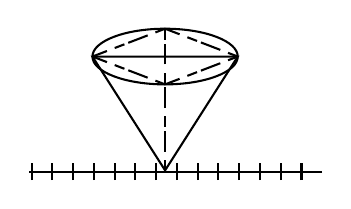
\begin{tikzpicture}[x=0.75pt,y=0.75pt,yscale=-1,xscale=1]
        \draw   (85,157.83) -- (120,103) -- (50,103) -- cycle ;
        \draw   (50,103) .. controls (50,95.59) and (65.67,89.59) .. (85,89.59) .. controls (104.33,89.59) and (120,95.59) .. (120,103) .. controls (120,110.41) and (104.33,116.41) .. (85,116.41) .. controls (65.67,116.41) and (50,110.41) .. (50,103) -- cycle ;
        \draw    (160.71,158.5) -- (19.29,158.5) (150.71,162.5) -- (150.71,154.5)(140.71,162.5) -- (140.71,154.5)(130.71,162.5) -- (130.71,154.5)(120.71,162.5) -- (120.71,154.5)(110.71,162.5) -- (110.71,154.5)(100.71,162.5) -- (100.71,154.5)(90.71,162.5) -- (90.71,154.5)(80.71,162.5) -- (80.71,154.5)(70.71,162.5) -- (70.71,154.5)(60.71,162.5) -- (60.71,154.5)(50.71,162.5) -- (50.71,154.5)(40.71,162.5) -- (40.71,154.5)(30.71,162.5) -- (30.71,154.5)(20.71,162.5) -- (20.71,154.5) ;
        \draw  [dash pattern={on 3.75pt off 3pt on 7.5pt off 1.5pt}]  (85,89.59) -- (50,103) ;
        \draw  [dash pattern={on 3.75pt off 3pt on 7.5pt off 1.5pt}]  (85,116.41) -- (50,103) ;
        \draw  [dash pattern={on 3.75pt off 3pt on 7.5pt off 1.5pt}]  (120,103) -- (85,116.41) ;
        \draw  [dash pattern={on 3.75pt off 3pt on 7.5pt off 1.5pt}]  (120,103) -- (85,89.59) ;
        \draw  [dash pattern={on 3.75pt off 3pt on 7.5pt off 1.5pt}]  (85,157.83) -- (85,89.59) ;
        \end{tikzpicture}
    \end{center}
    MIT Cheetah and other quadrupeds use QP-based MPC with linearized dynamics.
\end{itemize}

\section{Supplement 5}

\begin{itemize}
    \item Review on Julia array
    \item Introduction to Convex.jl
\end{itemize}

\section{Exercise 2}

\begin{itemize}
    \item Q1: Finite-Horizon LQR
    \item Q2: LQR for nonlinear systems
    \item Q3: Optimal rendezvous and docking 
\end{itemize}